\documentclass[english]{vaesen-supplement}
%% ================ TITLE ================ %%
\title{Vaesen\\LaTeX Template}
\titlepicture{img/lager-beer-frogs.jpg}
\subtitle{A \LaTeX-Template for Vaesen}
\author{Bulbafar \& Sibling Dex}
\introduction{
    This is a \LaTeX~ document class designed to create game supplements for the Vaesen RPG by Free League Publishing. 
}
\credits{    
    \textbf{ARTWORK:} 
    "Lager Beer Frogs" by Kennet Kjell Johansson Hultman,
    "The Jabberwocky" and "The White Rabbit" by John Tenniel,
    "Innkeeper" by Adrien Brouwer,
    "August Bebel" by unknown artist,
    "Krampus" by unknown artist (all Public Domain).

    \textbf{LICENCE:}
    This product was created under license. Vaesen and its logo are trademarks of Fria Ligan AB and Johan Egerkrans.

    This work contains material that is copyright Fria Ligan AB, Johan Egerkrans and/or other authors. Such material is used with permission under the Community Content Agreement for Free League Workshop.

    All other original material in this work is copyright \colorbox{yellow}{[year]} by \colorbox{yellow}{[your legal name or company name]} and published under the Community Content Agreement for Free League Workshop. 
}
%% ================ DOCUMENT ================ %%
\begin{document}
\maketitle

\tableofcontents

\chapter{About}

\section{This Template}
This \LaTeX-template is meant to replicate the \href{https://freeleaguepublishing.com/community-content/free-league-workshop/}{Free League Workshop} - Vaesen templates for Word and InDesign.


\section{Contact}
This template was made by \textbf{Bulbafar} and \textbf{Sibling Dex}. You can find us on the Vaesen RPG Discord server. Message us there if you are interested in helping with this project.

\begin{note}
\subsection{Work in Progess}

\begin{itemize}
    \item This template is work in progress!
    \bolditem{Last Updated:} 21 Sept. 2025
\end{itemize}

If you like to contribute, request features, or need help, contact us on the Vaesen RPG Discord server.
\end{note}

\parthead{
    \dragonpicture{img/Jabberwocky.jpg}
}
\part{Document Class Features}

\chapterhead{
\begin{quote}\handwritten
    "Quotes are useful to provide a short and flavourful introduction to a topic at the top of a new section or chapter."

    --The Author (always give credit)
\end{quote}
}
\chapter{Elements}

\noindent THIS DOCUMENT CLASS mimics the Vaesen template style provided by Free League for use with third-party Free League Workshop publications.

\section{Headings}
This document class provides styling for the heading types also used in \texttt{report} or \texttt{book} document classes.

\subsection{Parts}
The \verb|\part{...}| command generates a full-page heading with space for an image, as seen on the page before this one. 

Use the \verb|\parthead{...}| command to include an image or a text -- like an image using the \verb|\dragonpicture{...}| command as seen on top of the previous page. 

\subsection{Chapters}
The \verb|\chapter{...}| command produces a chapter heading, such as the one on this page. The chapter heading look like part headings, but are not placed on a separate page. 

You can use the \verb|\chapterhead{...}| command to include an image or a text -- like the note on this page. 


\subsection{Sections}
Use the \verb|\section{...}| command to generate section headings. This generates a one-column heading in the Berolina font. Use this to structure a chapter into the most important sections. 

\subsection{Subsections}
The \verb|\subsection{...}| command generates the bold-faced, centered heading you see above this paragraph. Use them to divide your longer texts into smaller chunks to provide orientation for the reader.

\subsubsection{Subsubsections}
The \verb|\subsubsection{...}| can be used if there is need to even further subdivide a subsection. This paragraph, for example, is under a subsubsection.

\subsection{Paragraphs}
The smallest defined division in this document class is the \verb|\paragraph{...}|. This command generated an inline bold heading that is best used for an unnumbered list of entries too long for an actual list environment.

\paragraph{This is a Paragraph:}
A nice way to use paragraphs is to add a colon at the end of the heading, as seen here.


\section{Lists}
The document class also modifies the standard list environments to match the Vaesen style.

\subsection{Itemize}
You can use a normal \verb|itemize| environment and \verb|\item| commands inside a list to produce a simple list entry.

\begin{itemize}
    \bolditem{Bold Item:} To add a bold keyword to the beginning of an item, use \verb|\bolditem{label}|.
    \coloritem{Color Item:} To make the bold keyword accent colored, use the \verb|\coloritem{label}| command.
    \coloritem[blue]{Color Item:}  You can make the keyword a custom color by the \verb|\coloritem[color]{label}| command. Specify the color in square brackets.
\end{itemize}

\subsection{Enumerate}
You can use a normal \verb|enumerate| environment and \verb|\item| commands inside a list to produce a numbered list entry.

\begin{enumerate}
    \item First list item.
    \item Second list item.
    \item Third list item.
\end{enumerate}

\section{Quote}
\begin{quote}
    This is a \verb|quote| environment, It can be used to place normal text, but is a great place to use the \verb|\handwritten| style:
    
    \handwritten This generates a handwritten text that looks like a letter or handwritten note.
\end{quote}


\section{Occult Symbols}
You can use the \verb|\bigsymbol{x}| command (using any ASCII character in it) to produce an occult symbol, like those on chapter headings or the note to the right.

\section{Package Options}
You can use all class options available to the standard \texttt{report} document class included in LaTeX.

%% ============================
\section{Boxes}

There are three types of box provided by this class: the \texttt{note} and \texttt{panel}. These are special environments that can be used to highlight special rules or important information in a compact way.

Use the \verb|\begin{panel}[options]{Heading}| environment to create a panel and the \verb|\begin{note}[options]{Heading}| environment to create a note (see examples below). Place the heading for the box in the second curly bracket and any optional commands in square brackets in between.

These boxes can be placed as one-column wide boxes in the flow of the text, or as floats by adding the \verb|[float*=h]| option (see more on the next page).

\begin{panel}{Panel}
    This is a \texttt{panel}, it can be used to highlight important information in a compact and noticeable way.
\end{panel}

\begin{note}[empty]{}
    \begin{center}
        \color{secret}
        \bigsymbol{e}
    \end{center}
    \heading{Note | Heading}    
    This is a \texttt{note}, they are used to emphasize information or add flavour text.
    You can add the \texttt{[empty]} option to the box to leave its top clear for a symbol (like here) and not add a pre-formatted heading.
\end{note}


\subsection{Wide Boxes}
Panels and notes can also be placed as wide, column-spanning boxes, for more explanations on how to do this, see the next section.

%% ========================================

%% ========================================
\chapter{Placement of Boxes}

\noindent THERE ARE SEVERAL methods to place narrow or wide boxes (notes or panels) on a page.
Placement of figures, panels, notes and tables can be tricky, especially if several of them has to go on the same page. This template uses the \verb|stfloat| package to help out, but fool around and find out is often needed. 

\begin{strip}
    \begin{panel}[wide]{Wide Panel using Strip}
        \begin{multicols}{2}%
            To generate a twocolumn layout in a wide box, wrap its content in a \verb|\begin{multicols}{2}| ... \verb|\end{multicols}| environment.
        \columnbreak
            \paragraph{Paragraph:}
            You can then use \verb|\columnbreak| to force a new column. Use other elements, like paragraphs, to further structure the box.
        \end{multicols}
    \end{panel}
\end{strip}

\subsection{Strip}
You can add a  \verb|\begin{strip}| ... \verb|\end{strip}| environment around a \verb|\begin{note}| or \verb|\begin{panel}| and \verb|[width=\textwidth]| in brackets to the box, to cut a wide box into the twocolumn page. See the example on this page. Beware that \verb|strip| is a bit buggy and only works correctly if immediately followed by text.

% You can add "float*=!t,width=\textwidth" in brackets to float a wide box on top of the page
\begin{note}[wide,float*=!b]
    \heading{Floating Wide Note}
    \begin{multicols}{2}
        Boxes, figures and tables can be positioned using !h (here), t (top) or b (bottom) in square brackets. Look up LaTeX floats for more information.
    \columnbreak
        \paragraph{Paragraph:}
        Doing so can be a little tricky, but the \verb|stfloats| package helps us here. Take a look at the code. 
    \end{multicols}
\end{note}

\newpage

\subsection{Floating}
You can add \verb|[wide,float*=!b]| in brackets to the \verb|\begin{note}| or \verb|\begin{panel}| to float it as a wide box on top of the page. See the note on the bottom of this page for example.

You can also, for example, add a \verb|[float=!b]| (without asterisk) to narrow boxes, to float them on the bottom of a page.

\cleardoublepage

\twocolumn[\section{Boxed Tables}]

\begin{panel}{Narrow Table}
    \begin{tabulary}{\linewidth}{C L}
        \textbf{D6} & \textbf{Result} \hphantom{Invisible text,   wider column} \\\hline %The hphantom can be used, as a less elegant way, to create the desired table with within the panel
        1 & What happens? \\
        2 & What happens? \\
        3 & What happens? \\
        4 & What happens? \\
        5 & What happens? \\
        6 & What happens?
    \end{tabulary}
\end{panel}

\begin{panel}[wide,float*=!b]{Table Panel}
\begin{tabulary}{\linewidth}{ c l c L }
    \textbf{DICE} & \textbf{LABEL} & \textbf{ALIGNMENT} & \textbf{DESCRIPTION} \\
    \hline
    1 & Dice & Center (c) & If you want a table to be rollable, use the first column as the die or dice column. Give it a header denoting the die/dice used, and number the rows. \\
    2 & Label & Left (l) & The first or second column of a table should be the label of the entry. This gives a short and meaningful name to the entry in the row. \\
    3 & Score & Center (c) & You can add several narrower columns for short, standardized scores, such as price, availability, durability, etc. \\
    4 & Description & Left (L) & The typically last column in a table is a longer description of the entry. Use a breaking alignment for this, so the description can be more than one line. \\
\end{tabulary}
\end{panel}

Lorem ipsum dolor sit amet, consectetur adipiscing elit. Nullam justo erat, sodales a aliquet eu, dignissim in lacus. Aliquam erat eros, viverra et ligula vel, mattis rutrum enim. Quisque ac arcu eu lorem tristique mollis eget aliquam nisl. Ut purus dolor, rhoncus et venenatis in, elementum vel lorem. Duis rutrum dolor in nulla luctus convallis. Donec cursus augue ipsum, quis hendrerit magna fringilla id. Mauris accumsan tempus molestie. Aenean in posuere tortor, in porta leo. Vestibulum pulvinar mauris eu dolor elementum dictum ut ut ligula. Suspendisse rutrum porta vestibulum. Donec vitae diam at metus ultricies dictum vel porttitor felis. Fusce eu est id neque tempus lacinia. Pellentesque faucibus nulla id nulla consectetur, eu laoreet dui gravida. Vestibulum sed consequat nunc. Vivamus vel consequat sem.

Nunc sed odio mattis, consectetur lorem in, vulputate sem. Etiam auctor condimentum ante, nec vulputate lectus facilisis et. Vestibulum et varius dui. Sed semper lectus quis dapibus sollicitudin. Nulla lectus lorem, consequat ut nibh a, porttitor mollis ex. Vestibulum tempus ut massa eu ultricies. Vivamus luctus vehicula erat quis convallis. Ut hendrerit in nunc sit amet commodo. Duis et turpis venenatis, consectetur orci sed, vestibulum massa. Quisque maximus faucibus justo quis laoreet. Class aptent taciti sociosqu ad litora torquent per conubia nostra, per inceptos himenaeos. Aliquam lobortis viverra urna, sit amet eleifend leo vulputate ut.

Phasellus est augue, maximus vel sapien sit amet, venenatis molestie arcu. Quisque ut eros metus. Sed mollis porttitor nibh et porttitor. Quisque iaculis nec mauris sed pulvinar. Nullam tristique ante sed lacinia commodo. Phasellus pretium lacus a libero iaculis.

%% ===========================
\parthead{\dragonpicture{img/white-rabbit.jpg}}
\part{Examples}

%===========================================
\chapter{Example Pages}

\noindent ON THE FOLLOWING pages, you can find some examples for archetypes, vaesen, or mysteries, to illustrate how this template can be used.

\cleardoublepage

\heading{Example Archetype:}
\section[Example Archetype]{\HUGE Innkeeper}

\begin{quote}\handwritten
    Here goes the description of an innkeeper, and why such a person can be a profession in a Vaesen game. This description could, of course, be a lot longer. Something along the lines of "there is an inn - a merry old inn"...   
\end{quote}
Lorem ipsum dolor sit amet, consectetur adipiscing elit. Mauris orci quam, ullamcorper a elit non, consectetur pulvinar metus. Ut tempor nisi ac felis cursus fermentum. Donec interdum urna at diam tempus feugiat non at nunc. Pellentesque egestas erat urna, et viverra lorem efficitur eu. Nam interdum et nisi posuere pharetra. Nunc sollicitudin maximus auctor. Aliquam magna augue, consequat non massa vel, bibendum tincidunt elit. Donec interdum urna at diam tempus feugiat non.

\begin{figure}[!b]
    \centering
    \fuzzyimage{img/Adriaen_Brouwer_-_Innkeeper.JPG}
    {\footnotesize "Innkeeper" by Adrien Brouwer (Public Domain)}
\end{figure}

\newpage

Choose among the suggestions and make up yourself

\subsubsection{Name}
\begin{itemize}
    \bolditem{First name:} Albertine, Bertil, Constance, Ib, Gertrud, Oluf 
    \bolditem{Last name}: Helmer, Jensen, Sand 
\end{itemize}
\subsubsection{Motivation}
\begin{itemize}
    \item Keeping people happy
    \item Earning money 
    \item Producing the finest beer
\end{itemize}
\subsubsection{Pride}
\begin{itemize}
    \item I have the best beer in town
    \item My father was a very famous whittler
    \item I once served the king
\end{itemize}
\subsubsection{Trauma}
\begin{itemize}
    \item A couple of trolls drank all my beer
    \item I took over the in from a lad caught by a spertus
    \item My mother have joined the sjörå after she gave birth to my sister. 
\end{itemize}
\subsubsection{Dark Secret}
\begin{itemize}
    \item I have to host a nisse party every year in the spring equinox
    \item I pay tribute to the local giant in beer and meat
    \item The gold I bought the inn for was stolen from a troll
\end{itemize}
\subsubsection{Relationships}
\begin{itemize}
    \item I like the way you talk
    \item I owe you much
    \item The one hand wash the other
\end{itemize}
\begin{panel}[empty]{}
\begin{itemize}
    \item \fakesc{Main Atribute}: Empathy
    \item \fakesc{Main Skill}: Observation
    \item \fakesc{Talents}: Would you like..., Clean up, Gossip
    \item \fakesc{Resources}: 2-6
    \item \fakesc{Equipment}: Cloth, Apron, Bottle of fine wine OR Spirits
\end{itemize}
\end{panel}

\newpage

\begin{strip}
\heading{Example Vaesen:}
\section[Example Vaesen]{\HUGE Krampus}

\begin{quote}\handwritten Lorem ipsum dolor sit amet, consectetur adipiscing elit. Mauris orci quam, ullamcorper a elit non, consectetur pulvinar metus. Ut tempor nisi ac felis cursus fermentum. Donec interdum urna at diam tempus feugiat non at nunc. Pellentesque egestas erat urna, et viverra lorem efficitur eu.\end{quote}
\end{strip}

Lorem ipsum dolor sit amet, consectetur adipiscing elit. Mauris orci quam, ullamcorper a elit non, consectetur pulvinar metus. Ut tempor nisi ac felis cursus fermentum. Donec interdum urna at diam tempus feugiat non at nunc. Pellentesque egestas erat urna, et viverra lorem efficitur eu.

\begin{figure}[!b]
    \centering
    \fuzzyimage{img/Krampus.jpg}
    {\footnotesize "Greetings from Krampus" by unknown artist, early 1900 (Public Domain)}
\end{figure}

\newpage

\begin{panel}{CHARACTERISTICS}
\fakesc{might}~10 \quad
\fakesc{body control}~8 \quad
\fakesc{magic}~5 \par
\fakesc{manipulation}~7 \quad
Fear~0
\end{panel}

\begin{note}
\heading{Secret}
    Here goes the secret of your vaesen. 
\end{note}

\begin{panel}{MAGICAL POWERS}
\begin{itemize}
    \item Enchant
    \item LaTeX Mastery
\end{itemize}
\end{panel}

Example of conflicts


\clearpage

\section{Example NPC}

\begin{center}
    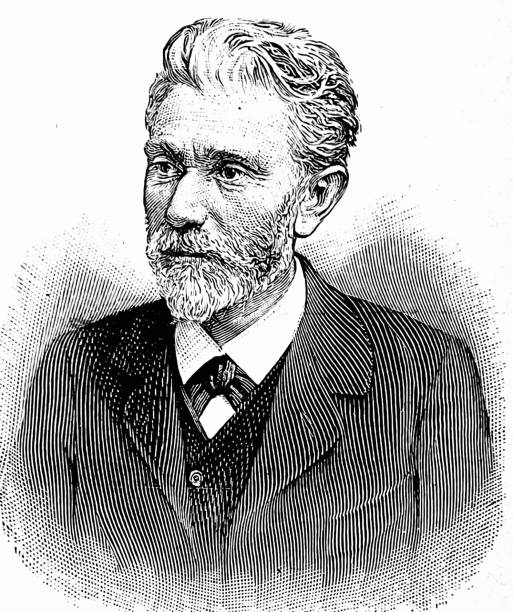
\includegraphics[width=0.8\linewidth]{img/Bebel.jpg}
    
    {\footnotesize "August Bebel" by unknown artist (1890, Public Domain)}
\end{center}

\begin{panel}[NPC]{John "The Bull" Doe}
    \NPCquote{"I will win the election, no matter what it takes!"}

    Lorem ipsum dolor sit amet, consectetur adipiscing elit. Nullam justo erat, sodales a aliquet eu, dignissim in lacus. Aliquam erat eros, viverra et ligula vel, mattis rutrum enim. Quisque ac arcu eu lorem tristique mollis eget aliquam nisl. Ut purus dolor, rhoncus et venenatis in, elementum vel lorem. Duis rutrum dolor in nulla luctus convallis. Donec cursus augue ipsum, quis hendrerit magna fringilla id. Mauris accumsan tempus molestie. Aenean in posuere tortor, in porta leo. Vestibulum pulvinar mauris eu dolor elementum dictum ut ut ligula. Suspendisse rutrum porta vestibulum. 

\begin{itemize}\sffamily\small
    \item Physique~1 \quad Precision~2 \quad Logic~2 \quad Empathy~3
    \item \fakesc{Inspiration}~3 \quad \fakesc{Observation}~3 \quad \fakesc{Medicine}~1
    \item Mental~Toughness~2 \quad Physical~Toughness~1
\end{itemize}
\end{panel}


\end{document}
